\documentclass[12pt]{article}
\newcommand{\gradeband}{Grades 4–5}
% Shared layout for the Week 7 student pages (compile with xelatex)
\usepackage[letterpaper, top=0.95in, bottom=0.75in, left=0.8in, right=0.8in,
            headheight=20pt, headsep=16pt, footskip=28pt]{geometry}
\usepackage{fontspec}
\setmainfont{Andika}
\usepackage{xcolor}
\usepackage{tikz}
\usetikzlibrary{arrows.meta,positioning,calc}
\usepackage[most]{tcolorbox}
\usepackage{fancyhdr}

\pagestyle{fancy}
\fancyhf{}
\lhead{\small Bellingham Math Circle \enspace\textperiodcentered\enspace Week 7
       \enspace\textperiodcentered\enspace \gradeband}
\rhead{\small Name \rule[-2pt]{5cm}{0.5pt}}
\cfoot{\small \thepage}
\renewcommand{\headrulewidth}{0.4pt}

\setlength{\parindent}{0pt}
\setlength{\parskip}{5pt}
\hyphenpenalty=10000
\exhyphenpenalty=10000
\AtBeginDocument{\raggedright}

\newcounter{prob}
\newcommand{\problem}{\stepcounter{prob}\par\textbf{Problem \theprob:}\enspace}

\newtcolorbox{rulebox}{enhanced, colback=white, colframe=black!55,
  boxrule=0.7pt, arc=2mm, left=8pt, right=8pt, top=6pt, bottom=6pt,
  before upper=\raggedright}

% ---- counters -------------------------------------------------------------
\tikzset{
  ctr/.style={circle, draw=black, fill=black!18, line width=0.6pt,
              minimum size=#1, inner sep=0pt},
  ctr/.default=5mm,
  xmark/.style={line width=1.4pt, line cap=round},
  ansbox/.style={draw=black, line width=0.6pt, minimum size=#1, inner sep=0pt},
  ansbox/.default=9mm,
}
% \pile[size]{n}{crossed}{per row}{step}  (drawn with top-left counter at origin)
\newcommand{\pile}[5][5mm]{%
  \foreach \i in {1,...,#2} {%
    \pgfmathtruncatemacro{\col}{mod(\i-1,#4)}%
    \pgfmathtruncatemacro{\row}{(\i-1)/#4}%
    \node[ctr=#1] (p\i) at (\col*#5, -\row*#5) {};%
    \pgfmathtruncatemacro{\thr}{#2-#3}%
    \ifnum\i>\thr
      \draw[xmark] ($(p\i)+(-0.62*#1,0.62*#1)$) -- ($(p\i)+(0.62*#1,-0.62*#1)$)
                   ($(p\i)+(0.62*#1,0.62*#1)$) -- ($(p\i)+(-0.62*#1,-0.62*#1)$);
    \fi
  }}


% label table: \labtable{first}{last} in rows of 10
\newcommand{\labtable}[2]{%
  \begin{tikzpicture}[x=1.62cm, y=1cm]
    \foreach \n in {#1,...,#2} {
      \pgfmathtruncatemacro{\k}{\n-#1}
      \pgfmathsetmacro{\cx}{mod(\k,10)}
      \pgfmathsetmacro{\cy}{-2.2*int(\k/10)}
      \fill[black!10] (\cx,\cy) rectangle ++(1,-0.75);
      \draw[line width=0.6pt] (\cx,\cy) rectangle ++(1,-0.75);
      \draw[line width=0.6pt] (\cx,\cy-0.75) rectangle ++(1,-1.05);
      \node[font=\bfseries, text height=1.6ex, text depth=0.2ex] at (\cx+0.5,\cy-0.375) {\n};
    }
  \end{tikzpicture}}

\newcommand{\moves}[1]{\{#1\}}

\begin{document}
\fontsize{12.5}{17.5}\selectfont
\setlength{\parskip}{6pt}

\begin{rulebox}
A take-away game uses one pile of counters and a set of allowed moves, such as
\moves{1, 3, 4}. Two players take turns. On each turn a player removes a number
of counters that is in the set, and no more than the pile has. Whoever takes
the last counter wins.

\smallskip
A pile is a \textbf{losing pile} (L) if the player about to move will lose when
the other player plays carefully. Every other pile is a \textbf{winning pile}
(W). A pile of 0 is a losing pile, because the other player has just taken the
last counter.
\end{rulebox}

\medskip
\problem Allowed moves \moves{1, 2}. Describe all the losing piles, and explain
why your description is correct for piles of every size.

\vspace{5.4cm}

\problem Allowed moves \moves{1, 3, 4}. Label each pile from 0 to 29 with W or
L. Describe all the losing piles, and explain why your description is correct
for piles of every size.

\medskip
\begin{center}
\labtable{0}{29}
\end{center}

\vfill
\newpage

\problem Allowed moves \moves{1, 3, 4}. A player always takes as many counters
as the rules allow. This player moves first, and the opponent plays carefully.
From which piles does this player win?

\vspace{8.8cm}

\problem Allowed moves \moves{1, 3, 5}. Describe all the losing piles. Find
every set of allowed moves that contains 1 and has exactly the same losing
piles as \moves{1, 3, 5}.

\vfill
\newpage

\problem Allowed moves \moves{1, 2, \textit{m}}, where \textit{m} is a whole
number larger than 2. For which \textit{m} are the losing piles exactly the
multiples of 3, as they are for \moves{1, 2}? For every other \textit{m},
describe the losing piles.

\vspace{6.6cm}

\problem Allowed moves \moves{1, 6, 9}. Label each pile from 0 to 39 with W or
L. From some pile on, the labels repeat in a cycle forever. Find the pile
where the repeating starts and the length of the cycle.

\medskip
\begin{center}
\labtable{0}{39}
\end{center}

\vfill
\newpage

\problem Explain why, for every finite set of allowed moves, the labels W and
L eventually repeat in a cycle forever.

\vspace{7.4cm}

\begin{rulebox}
In a game with two piles, a player chooses one pile on each turn and removes
an allowed number of counters from that pile only. Whoever takes the last
counter wins.

\smallskip
Give each single pile a \textbf{value}. A pile of 0 has value 0. The value of
any other pile is the smallest whole number that is not the value of a pile
you can reach from it in one move.
\end{rulebox}

\problem Allowed moves \moves{1, 3, 4}. Find the value of each pile from 0 to
20.

\medskip
\begin{center}
\labtable{0}{20}
\end{center}

\vfill
\newpage

\problem Allowed moves \moves{1, 3, 4}, with two piles. For each pair of
piles, decide whether the player about to move can win. When that player can
win, find a winning first move.

\medskip
\begin{center}
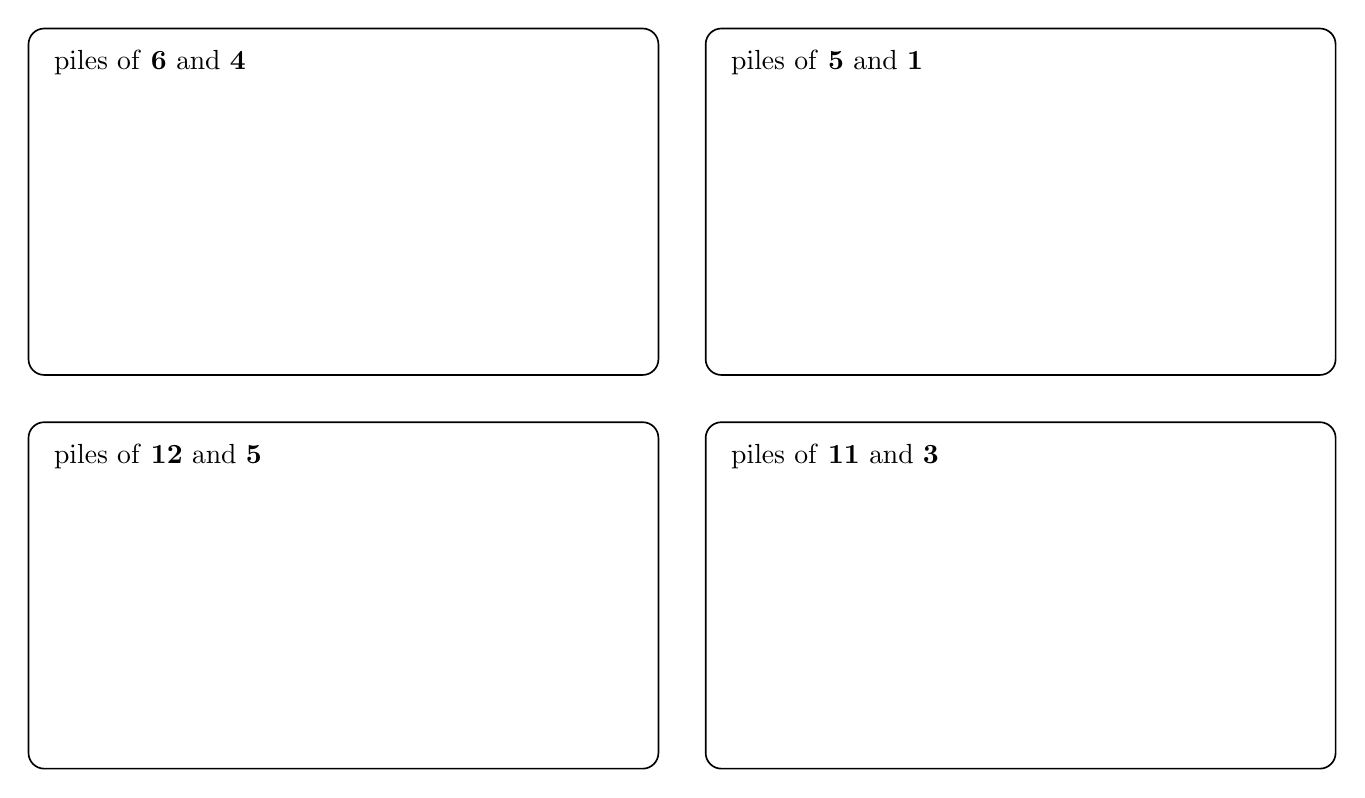
\begin{tikzpicture}
  \foreach \a/\b/\x/\y in {6/4/0/0, 5/1/8.6/0, 12/5/0/-5.0, 11/3/8.6/-5.0} {
    \draw[rounded corners=2mm, line width=0.6pt] (\x,\y) rectangle ++(8,-4.4);
    \node[anchor=north west] at (\x+0.2,\y-0.15) {piles of \textbf{\a} and \textbf{\b}};
  }
\end{tikzpicture}
\end{center}

\vspace{0.6cm}
\problem Explain why, with two piles, the player about to move loses against
careful play when the two values are equal, and can win when the two values
are different.

\vfill
\end{document}
